\documentclass{article}
\usepackage{pgf}
\usepackage{tikz}
\usetikzlibrary{arrows,automata}
\usepackage[latin1]{inputenc}
\usepackage{listings}
\lstdefinestyle{customc}{
  belowcaptionskip=1\baselineskip,
  breaklines=true,
  frame=L,
  xleftmargin=\parindent,
  language=C,
  showstringspaces=false,
  basicstyle=\footnotesize\ttfamily,
  keywordstyle=\bfseries\color{green!40!black},
  commentstyle=\itshape\color{purple!40!black},
  identifierstyle=\color{blue},
  stringstyle=\color{orange},
}
\lstset{escapechar=@,style=customc}

\newcommand\D{4}

\begin{document}

\begin{figure}
\center
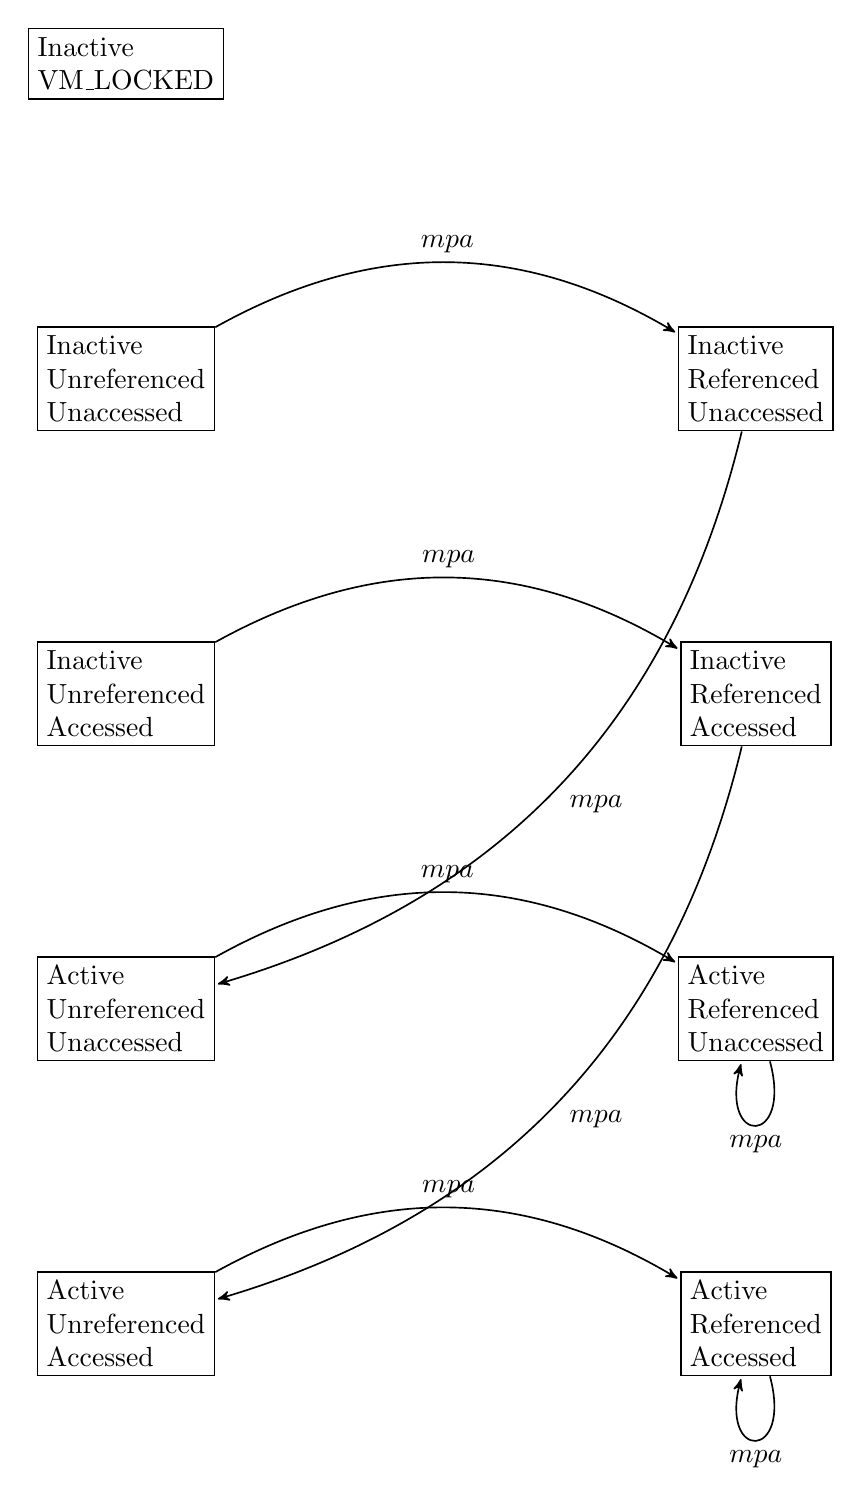
\begin{tikzpicture}[->,>=stealth',shorten >=1pt,auto,node distance=\D{}cm,
                    semithick]

  \tikzstyle{every state}=[rectangle,draw,align=left]

  \node[state] (IUU) at (0,0)        {Inactive \\ Unreferenced \\ Unaccessed};
  \node[state] (IRU) at (2*\D,0)     {Inactive \\ Referenced   \\ Unaccessed};
  \node[state] (LCK) at (0,\D)       {Inactive \\ VM\_LOCKED};
  \node[state] (IUA) at (0,-\D)      {Inactive \\ Unreferenced \\ Accessed};
  \node[state] (IRA) at (2*\D,-\D)   {Inactive \\ Referenced   \\ Accessed};
  %\node[state] (IAA) at (\D,-\D)     {Inactive \\ Unreferenced \\ Accessed $>$ 1};
  \node[state] (AUU) at (0,-2*\D)    {Active   \\ Unreferenced \\ Unaccessed};
  \node[state] (ARU) at (2*\D,-2*\D) {Active   \\ Referenced   \\ Unaccessed};
  \node[state] (AUA) at (0,-3*\D)    {Active   \\ Unreferenced \\ Accessed};
  \node[state] (ARA) at (2*\D,-3*\D)  {Active   \\ Referenced   \\ Accessed};


\path
(IUU) edge [bend  left] node {$mpa$} (IRU)
(IRU) edge [bend  left] node {$mpa$} (AUU)
(IUA) edge [bend  left] node {$mpa$} (IRA)
(IRA) edge [bend  left] node {$mpa$} (AUA)
%(IAA) edge [bend left] node {$mpa$} ()
(AUU) edge [bend  left] node {$mpa$} (ARU)
(ARU) edge [loop below] node {$mpa$} (ARU)
(AUA) edge [bend  left] node {$mpa$} (ARA)
(ARA) edge [loop below] node {$mpa$} (ARA)
;
\end{tikzpicture}
\end{figure}

\begin{figure}
\center
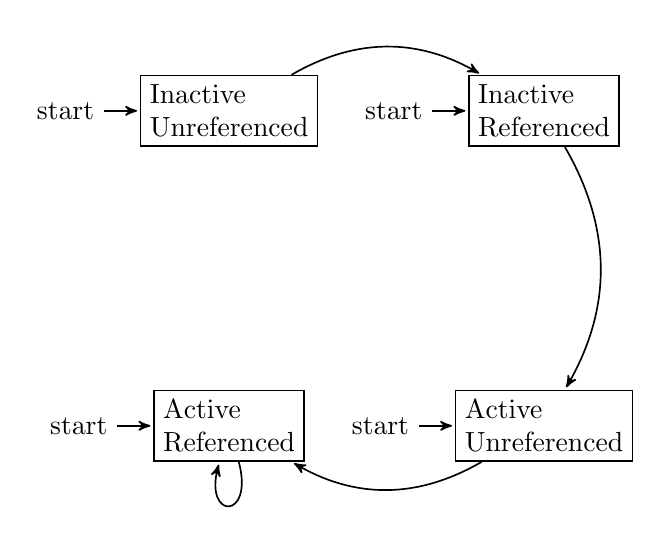
\begin{tikzpicture}[->,>=stealth',shorten >=1pt,auto,node distance=4cm,
                    semithick]

  \tikzstyle{every state}=[rectangle,draw,align=left]

  \node[initial,state] (IU)               {Inactive \\ Unreferenced};
  \node[initial,state] (IR) [right of=IU] {Inactive \\ Referenced};
  \node[initial,state] (AU) [below of=IR] {Active \\ Unreferenced};
  \node[initial,state] (AR) [below of=IU] {Active \\ Referenced};

  \path (IU) edge [bend  left] node {} (IR)
        (IR) edge [bend  left] node {} (AU)
        (AU) edge [bend  left] node {} (AR)
        (AR) edge [loop below] node {} (AR);
\end{tikzpicture}
\caption{Classic}
\end{figure}
\begin{figure}
\center
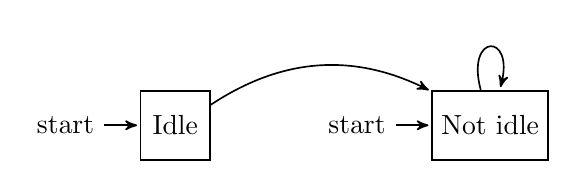
\begin{tikzpicture}[->,>=stealth',shorten >=1pt,auto,node distance=4cm,
                    semithick]

  \tikzstyle{every state}=[rectangle,draw,align=left]

  \node[initial,state] (IL)               {Idle};
  \node[initial,state] (NI) [right of=IL] {Not idle};

  \path (IL) edge [bend  left] node {} (NI)
        (NI) edge [loop above] node {} (NI);
\end{tikzpicture}
\caption{Idle page tracking}
\end{figure}
\lstinputlisting[caption=mark\_page\_accessed, style=customc]{src/mark_page_accessed.c}
\end{document}
